
This chapter describes the overall architecture and design of the EpiDetect system. The discussion covers the end-to-end processing pipeline, the data flow through the system, and the design of each individual module. Each diagram is intentionally placed alongside the descriptive text that introduces it, so the reader does not have to flip pages to follow the design.

\section{System Architecture Overview}

The EpiDetect system follows a modular, layered architecture where each processing stage is encapsulated in its own module. Data flows sequentially from raw EEG input through preprocessing, feature extraction, classification, and explanation. The overall architecture is presented in Figure~\ref{fig:sysarch}.

The architecture in Figure~\ref{fig:sysarch} is significant because it makes the boundary between the offline training pipeline (top vertical chain) and the online inference path (the Flask REST API and Web Dashboard at the bottom) explicit. The trained ensemble in the centre is the single artifact shared between the two paths, which is why the SHAP explainer attaches to it directly rather than to the raw signal.

\begin{figure}[ht]
\centering
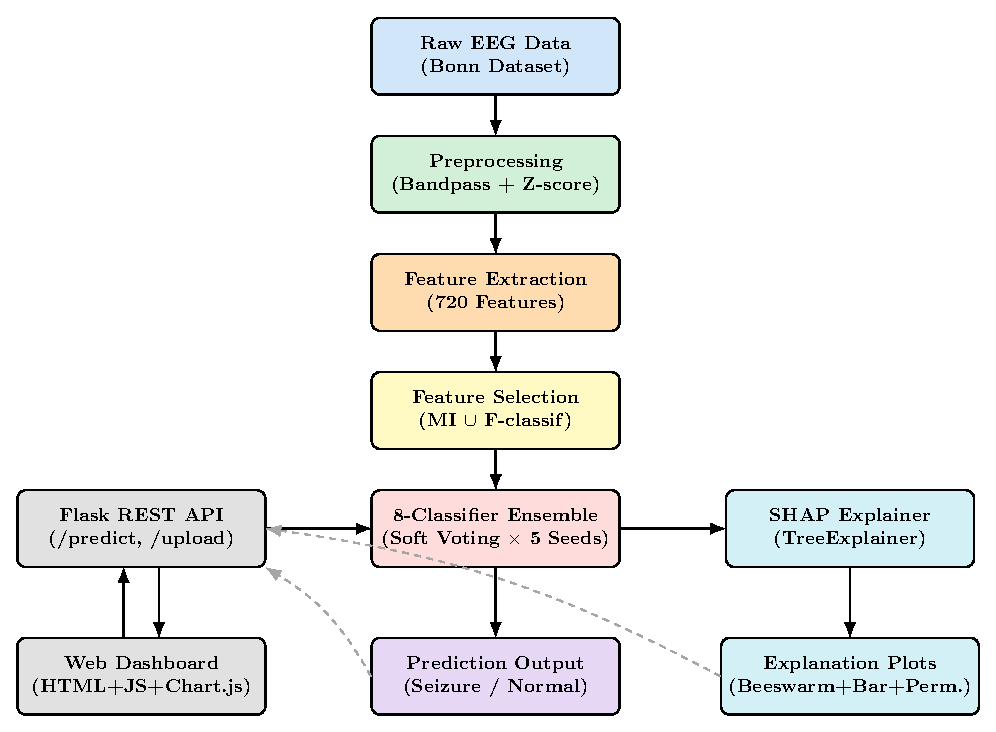
\includegraphics[width=0.78\textwidth]{images/sys_architecture.pdf}
\caption{System Architecture of the EpiDetect Pipeline.}
\label{fig:sysarch}
\end{figure}

\section{Process Flow of the Pipeline}

Figure~\ref{fig:processflow} illustrates the end-to-end process flow from the moment a user submits an EEG signal to the point where a prediction and explanation are displayed. Unlike the architectural view in Figure~\ref{fig:sysarch}, which captures the static layering of components, the process flow emphasises the temporal order in which each stage runs at inference time. This is important because each stage strictly depends on the output of the previous one; a missing or malformed intermediate output halts the pipeline.

\begin{figure}[H]
\centering
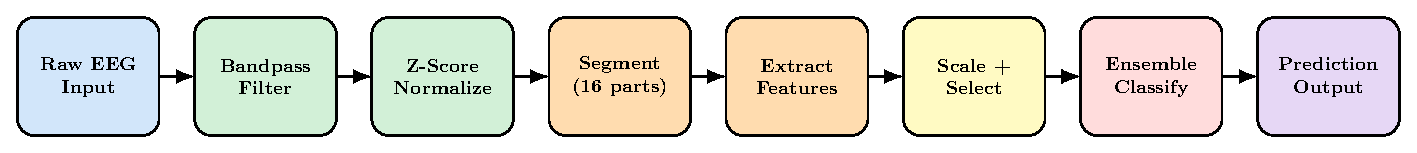
\includegraphics[width=\textwidth]{images/process_flow.pdf}
\caption{Process Flow Diagram: end-to-end signal processing pipeline.}
\label{fig:processflow}
\end{figure}

\section{Data Flow Diagram}

Figure~\ref{fig:dfd} presents a Level-1 data flow diagram showing how data moves between the major components of the system. The diagram makes two design properties visible at a glance. First, the trained model store (D2) feeds only the classification process and not the feature extractor, which is exactly the runtime relationship: features are computed from the input signal, while weights are loaded into the classifier. Second, the explanation process (4.0) closes the loop by routing both the prediction and its SHAP-based justification back to the user, which is the project's contribution toward clinical transparency.

\begin{figure}[H]
\centering
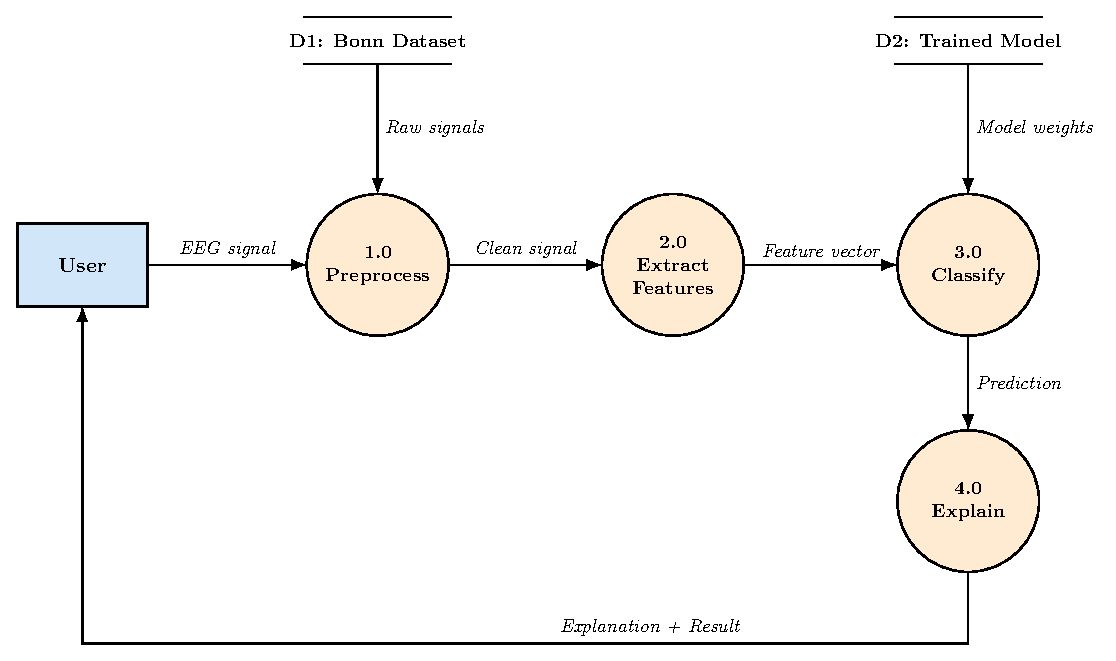
\includegraphics[width=0.95\textwidth]{images/dfd.pdf}
\caption{Level-1 Data Flow Diagram (Yourdon notation).}
\label{fig:dfd}
\end{figure}

\section{Activity Diagram}

Figure~\ref{fig:activity} presents the activity diagram for the EpiDetect prediction workflow, showing the sequence of operations along with the two key decision points that govern the processing path. The first decision (\textit{Valid Signal?}) acts as an input guard, returning an error before any processing if the uploaded file is malformed; this protects the downstream stages from spurious computation. The second decision (\textit{Prob $\geq 0.5$?}) converts the ensemble's continuous probability output into the binary clinical label that the dashboard displays. Note that the activity diagram intentionally treats the eight-classifier ensemble and the five-seed averaging as a single atomic activity (\textit{Run Ensemble (5 Seeds)}), because at the workflow level the user does not distinguish between the constituent classifiers. The internal structure of that activity is documented separately in the ensemble classification module design (Section~4.7.5).

\begin{figure}[H]
\centering
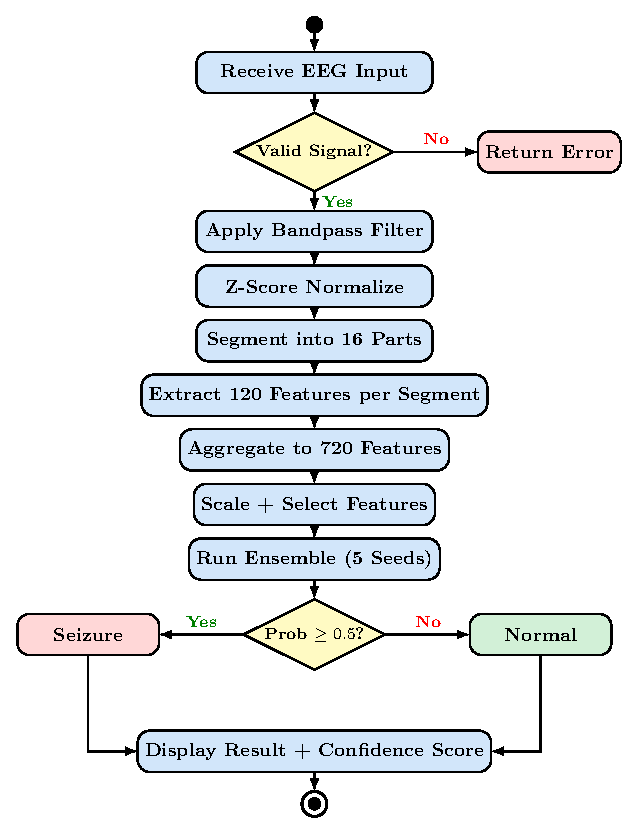
\includegraphics[width=0.55\textwidth]{images/activity_diagram.pdf}
\caption{Activity Diagram: EEG Prediction Workflow.}
\label{fig:activity}
\end{figure}

\section{Sequence Diagram}

Figure~\ref{fig:sequence} illustrates the interaction between the main components of the system during a typical prediction request. The user initiates a file upload through the browser, which communicates with the Flask API. The API delegates processing to the backend modules in sequence and returns the final result. The diagram is significant in two ways. First, it identifies the Flask API as the single orchestrator at inference time: every component except the User and Frontend communicates only through the API, which keeps the frontend stateless and the backend modules independently testable. Second, it makes the synchronous nature of the request-response cycle explicit: the API blocks on each backend stage in turn, so an error or delay in any one stage immediately surfaces in the JSON response delivered to the user. The dashed return arrows show that responses follow the inverse of the call chain, which means there is no out-of-band notification path; everything the user sees comes from the single response to the original POST request.

\begin{figure}[H]
\centering
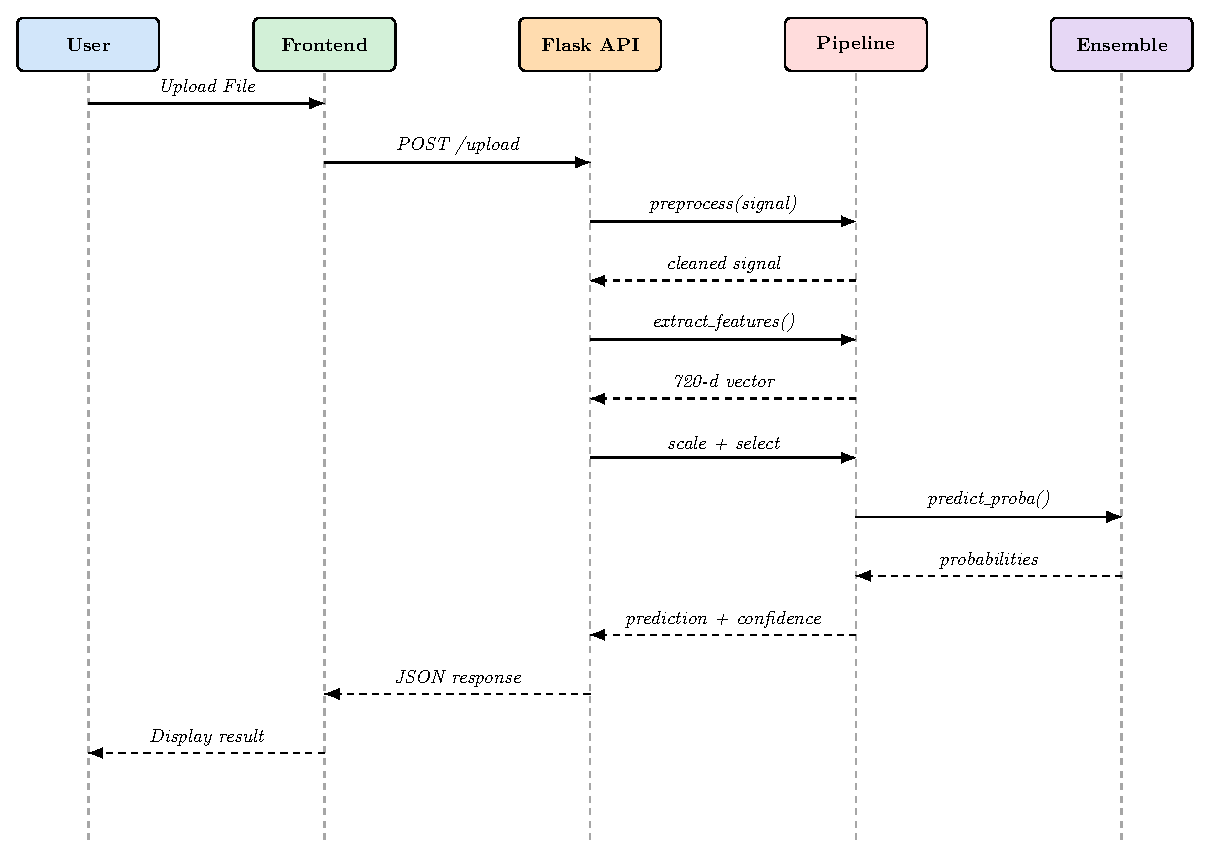
\includegraphics[width=\textwidth]{images/sequence_diagram.pdf}
\caption{Sequence Diagram: Signal Upload and Prediction.}
\label{fig:sequence}
\end{figure}

\section{Module Dependency Diagram}

Figure~\ref{fig:moduledep} shows the dependency relationships between the backend Python modules. The graph is deliberately a directed acyclic graph: \texttt{main.py} (the training entry point) depends only on the \texttt{cross\_validation} orchestrator, while \texttt{app.py} (the Flask inference entry point) depends on the four modules it directly invokes at runtime, namely \texttt{preprocess}, \texttt{extract}, \texttt{ensemble}, and \texttt{explainer}. The four worker modules and the \texttt{loader} all import constants from \texttt{settings} (paths, hyperparameters, feature counts), so each of them has an outgoing edge into \texttt{settings} at the bottom of the diagram. Every other module depends downward only, and \texttt{settings} has zero outgoing edges. This layered structure was chosen because it allows any individual module to be swapped (for example, replacing the ensemble with a different classifier) without recompiling or modifying any other module.

\begin{figure}[H]
\centering
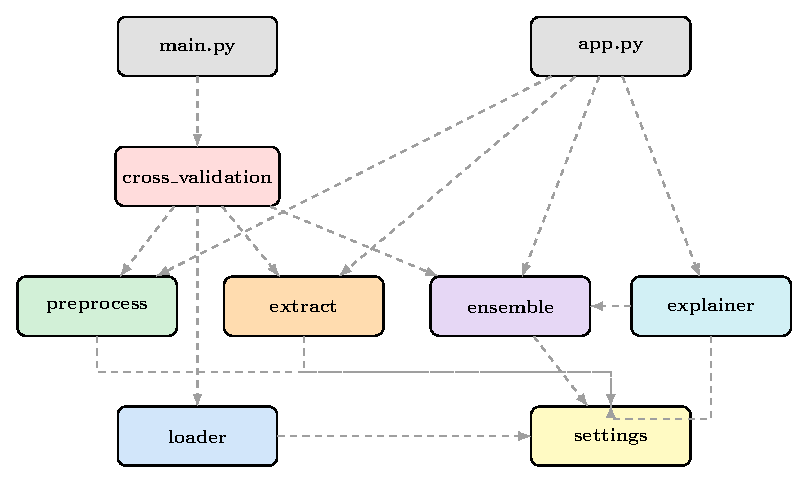
\includegraphics[width=0.85\textwidth]{images/module_dependency.pdf}
\caption{Module Dependency Diagram.}
\label{fig:moduledep}
\end{figure}

\section{Module Design}

This section describes the design of each module in the pipeline.

\subsection{Data Loading Module}

The data loader reads the Bonn University EEG dataset from disk. Each of the five clinical sets (Z, O, N, F, S) is stored as a collection of text files, where each file contains 4097 amplitude values sampled at 173.61~Hz. The loader scans the dataset directory, identifies each set by its starting letter, reads all files in that set, and assigns the appropriate binary label (0 for non-seizure, 1 for seizure).

\subsection{Preprocessing Module}

The preprocessing module applies two transformations to each raw signal. First, a fourth-order Butterworth bandpass filter with cutoff frequencies at 0.5~Hz and 85~Hz removes DC drift and high-frequency noise. The filter is applied using zero-phase filtering (\texttt{filtfilt}) so that no time delay is introduced. Second, z-score normalization is applied to standardize each signal to zero mean and unit variance. This ensures that the feature extraction pipeline receives signals on a consistent scale.

\subsection{Feature Extraction Module}

This module is the most computationally intensive part of the pipeline. Each signal (4097 samples) is split into 16 equal segments. For each segment, 120 features are computed across four domains:

\begin{enumerate}
    \item \textbf{DWT Features:} Five sub-bands (one approximation, four detail levels) each described by 15 statistics: mean, max, min, variance, wavelet entropy, energy, max absolute, min absolute, standard deviation, kurtosis, skewness, RMS, zero-crossing rate, mean absolute deviation, and coefficient of variation.

    \item \textbf{Time-Domain Features:} Mean, standard deviation, max, min, peak-to-peak range, kurtosis, skewness, RMS, zero-crossing rate, mean absolute value, Hjorth mobility, Hjorth complexity, line length, Teager energy, IQR, median absolute deviation, and variance.

    \item \textbf{Frequency-Domain Features:} Total power, peak frequency, mean frequency, median frequency, spectral entropy, absolute and relative band powers for delta through gamma, theta/alpha ratio, delta/beta ratio, slow/fast ratio, spectral edge frequencies at 85\% and 95\%, spectral centroid, and spectral spread.

    \item \textbf{Nonlinear Features:} Sample entropy, permutation entropy (orders 3 and 4), detrended fluctuation analysis (DFA), Higuchi fractal dimension, and a rescaled-range Hurst exponent estimate.
\end{enumerate}

After computing 120 features per segment across 16 segments, the values are aggregated using six statistics: mean, standard deviation, maximum, minimum, median, and interquartile range. This yields $120 \times 6 = 720$ features per signal.

Figure~\ref{fig:featurearch} shows the feature extraction architecture. The diagram is important for understanding the dimensionality bookkeeping: the 720 figure quoted throughout this report is not arbitrary, but the product of 120 per-segment features and 16 segments, summarised through 6 aggregation statistics. Any change to one of these three numbers propagates to the final feature count.

\begin{figure}[H]
\centering
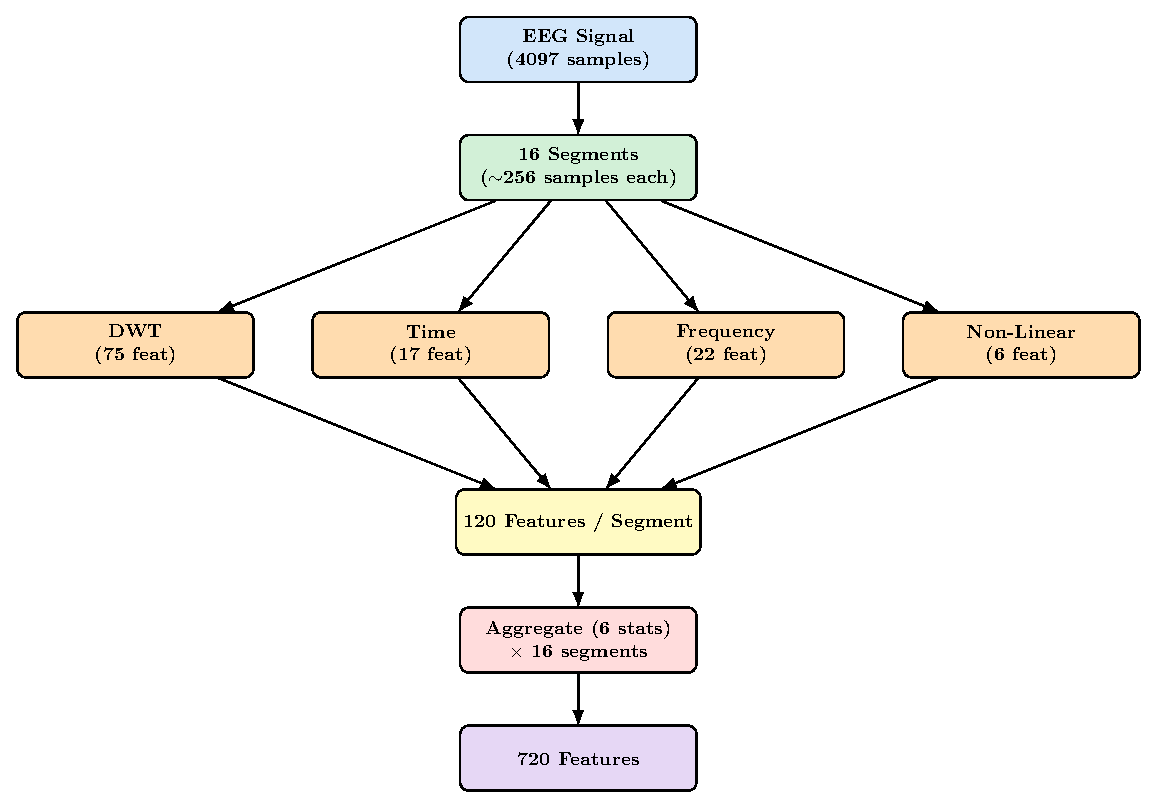
\includegraphics[width=0.7\textwidth]{images/feature_arch.pdf}
\caption{Feature Extraction Architecture.}
\label{fig:featurearch}
\end{figure}

\subsection{Feature Selection Module}

The feature selection module applies a union-based strategy. Two separate selectors, Mutual Information and ANOVA F-classif, each identify the top-$k$ (200) most informative features. The union of both sets is taken, yielding a feature subset that retains any feature considered important by \textit{either} method. This typically produces a subset of 280 to 330 features, which is considerably smaller than the original 720 but retains a broader view of relevance than a single selector alone.

\subsection{Ensemble Classification Module}

The classification module constructs a soft-voting ensemble of eight classifiers. Each classifier brings a different inductive bias, summarised in Table~\ref{tab:classifiers}. The table is important because it makes explicit \textit{why} eight different classifiers are combined rather than simply tuning a single one: each row identifies a distinct learning bias, and the soft-voting scheme ensures that no single bias dominates the final probability estimate.

\begin{table}[htbp]
\centering
\renewcommand{\arraystretch}{1.3}
\caption{Eight Classifiers in the Ensemble.}
\label{tab:classifiers}
\resizebox{\textwidth}{!}{%
\begin{tabular}{|c|p{5cm}|p{8.5cm}|}
\hline
\textbf{No.} & \textbf{Classifier} & \textbf{Role in the Ensemble} \\
\hline
1 & Random Forest (RF) & Bagging ensemble; robust, low variance. \\
\hline
2 & Extra Trees (ET) & More randomized than RF; further reduces overfitting. \\
\hline
3 & Hist. Gradient Boosting (HGB) & Fast boosting algorithm; handles large feature sets. \\
\hline
4 & Gradient Boosting (GBM) & Sequential boosting; corrects residual errors. \\
\hline
5 & AdaBoost & Focuses on hard to classify samples. \\
\hline
6 & SVM (RBF kernel) & Finds optimal decision boundaries in high-dimensional space. \\
\hline
7 & MLP (Neural Network) & Learns nonlinear feature combinations. \\
\hline
8 & K-Nearest Neighbours (KNN) & Captures local neighbourhood patterns. \\
\hline
\end{tabular}%
}
\end{table}

The ensemble uses \textit{soft voting}: each classifier outputs a probability for the seizure class, and the final probability is the average across all eight. To further reduce variance, the entire ensemble is trained five times with different random seeds, and the final prediction is the average of all five runs.

\subsection{XAI Module}

The explainability module uses SHAP (SHapley Additive exPlanations)~\citep{lundberg2017unified} to provide three types of explanations:

\begin{enumerate}
    \item \textbf{Global Feature Importance:} Averaged across all tree-based estimators in the ensemble, this shows which features the model relies on most heavily overall.

    \item \textbf{SHAP Summary and Bar Plots:} Multi-tree SHAP values are computed by averaging TreeExplainer outputs from the Random Forest, Extra Trees, and Gradient Boosting components. The summary beeswarm plot shows how each feature's value influences the prediction across all test samples, while the bar plot ranks features by mean absolute SHAP value.

    \item \textbf{Permutation Importance:} Each feature's values are randomly shuffled and the resulting drop in accuracy is measured using the full eight-classifier ensemble, revealing which features are genuinely critical to the model's performance.
\end{enumerate}

\subsection{REST API and Web Dashboard}

The Flask-based REST API serves as the bridge between the trained model and the user-facing dashboard. It exposes endpoints for health checking, signal prediction, file upload, and XAI plot retrieval. The frontend, built with vanilla HTML, CSS, and JavaScript (with Chart.js for data visualization), connects to these endpoints and presents predictions, confidence scores, and explanation plots in an interactive interface.

\section{Project Directory Structure}

Table~\ref{tab:dirstructure} shows the modular directory organization of the codebase. The structure mirrors the module dependency diagram in Figure~\ref{fig:moduledep}: each row corresponds to a node in the graph, and the directory hierarchy reflects the layered grouping (configuration at the top, workers in the middle, entry points at the bottom).

\begin{table}[htbp]
\centering
\renewcommand{\arraystretch}{1.15}
\caption{Project Directory Structure.}
\label{tab:dirstructure}
\resizebox{\textwidth}{!}{%
\begin{tabular}{|p{7cm}|p{7cm}|}
\hline
\textbf{Path} & \textbf{Purpose} \\
\hline
\texttt{backend/config/settings.py} & All constants and hyperparameters \\
\hline
\texttt{backend/data/loader.py} & Bonn dataset loader \\
\hline
\texttt{backend/preprocessing/preprocess.py} & Bandpass filter + z-score normalization \\
\hline
\texttt{backend/features/extract.py} & 720 feature extraction pipeline \\
\hline
\texttt{backend/models/ensemble.py} & 8 classifier soft-voting ensemble \\
\hline
\texttt{backend/training/cross\_validation.py} & 10-fold CV + model saving \\
\hline
\texttt{backend/xai/explainer.py} & SHAP-based explanations \\
\hline
\texttt{backend/main.py} & Full training pipeline entry point \\
\hline
\texttt{backend/app.py} & Flask REST API \\
\hline
\texttt{frontend/index.html} & Web dashboard \\
\hline
\texttt{frontend/js/app.js} & Frontend logic + Chart.js \\
\hline
\texttt{frontend/css/style.css} & Dashboard styling \\
\hline
\end{tabular}%
}
\end{table}
